\documentclass{standalone}

\usepackage{tikz}

\usepackage{graphicx}
\usetikzlibrary{angles, quotes}
	\usetikzlibrary{arrows.meta, positioning, quotes, shapes, shapes.geometric}
	\definecolor{baseline6}{HTML}{6940FF}
	\definecolor{baseline5}{HTML}{A12EFF}
	\definecolor{baseline4}{HTML}{D24AFF}
	\definecolor{baseline3}{HTML}{FF7DF0}
	\definecolor{baseline2}{HTML}{FFBDD4}
	
	\definecolor{thick6}{HTML}{00BDA8}
	\definecolor{thick2}{HTML}{77F3DB}
	
	\definecolor{thin6}{HTML}{D47E04}
	\definecolor{thin2}{HTML}{FFDA09}
	
	\definecolor{single}{HTML}{00A2FF}
	\definecolor{full}{HTML}{425df5}
	
	\definecolor{expt1col}{HTML}{FF0099}
	\definecolor{expt3col}{HTML}{527319}
	\definecolor{expt2col}{HTML}{0000FF}
	\tikzset{nodes={font=\sffamily}} 
	\tikzset{
		axis/.style={nodes={font=\sffamily, fill=gray!40, fill opacity=.5, text opacity =1, inner sep=4pt, outer sep=3pt, anchor=text, rectangle, rounded corners}},
		expt1/.style={
			draw, circle, color=expt1col, line width=0, align=center, scale=1.5, font=\sffamily},
		expt2/.style={
			draw, circle, color=expt2col, line width=0,  align=center, scale=1.5, font=\sffamily},
		expt3/.style={
			draw, circle, color=expt3col, line width=0, align=center, scale=1.5, font=\sffamily},
		illus/.style={draw, rectangle, align=center},
		annotate/.style={
			color=black!60, line width=0, align=center, scale=1, font=\sffamily},
		illus/.style={draw, rectangle, rounded corners, minimum height=7em, align=center, color=black!50, font=\sffamily, scale=1},
		bound/.style={draw, rectangle, align=center, color=black, font=\sffamily, scale=1},
		toplabel/.style={font=\sffamily, fill=gray!40, fill opacity=.5, text opacity =1, inner sep=4pt, outer sep=3pt, anchor=text, rectangle, rounded corners}
	}
	
\begin{document}
\begin{tikzpicture}
		


	%	\node at (13,4) {\LARGE\bfseries{C}};

		\def\r{4}
		\def\t{3}
		\def\bx{9}
		\def\by{0}
		
		\def\ax{-12}
		\def\ay{.5}
		
		\def\clabx{-4.5}
		\def\claby{-6}
		\def\clabz{-8.7}
		
		\def\cola{-3}
		\def\colb{1.5}
		\def\colc{7}
		\def\cold{11.5}
		
		
		\node at (\bx+-3.5,\by+5) {\LARGE\bfseries{B}};
		\node at (\ax+7,\ay+4.5) {\LARGE\bfseries{A}};
		\node at (\cola-2,\clabx+.2) {\LARGE\bfseries{C}};
		
		\draw (\bx,\by) edge[-Stealth, line width=1] [axis, "Matcher Contributions", sloped, pos=.55] (\bx-\r/1.4,  \by-\r/1.4) ;
		\draw (\bx,\by) edge[-Stealth, line width=1] [axis, "Group Size", pos=1.05] (\bx+\r, \by) ;
		\draw (\bx,\by) edge[-Stealth, line width=1] [axis, "Group coherence", sloped, pos=.45] (\bx, \by+\r);
		\draw[dashed] (\bx+\t,\by) edge [] (\bx+\t-\t/1.4, \by-\t/1.4);
		\draw[dashed] (\bx-\t/1.4,\by-\t/1.4) edge [] (\bx+\t-\t/1.4, \by-\t/1.4);
		\draw[dashed] (\bx,\by+\t) edge [] (\bx+\t,\by+\t);
		\draw[dashed] (\bx+\t,\by) edge [] (\bx+\t+.2,\by+\t/2-.2);
		\draw[dashed] (\bx+\t,\by) edge [] (\bx+\t-.2,\by+\t/2+.2);
		\draw[dashed] (\bx+\t,\by+\t) edge [] (\bx+\t+.2,\by+\t/2-.2);
		\draw[dashed] (\bx+\t,\by+\t) edge [] (\bx+\t-.2,\by+\t/2+.2);
		
		\node (n2) at (\bx,\by) [expt1, fill=expt1col, label={[expt1col]below:2}] {};
		\node (n3) at (\bx+\t/4,\by) [expt1, fill=expt1col, label={[expt1col]below:3}] {};
		\node (n4) at (\bx+\t/2,\by) [expt1, fill=expt1col, label={[expt1col]below:4}] {};
		\node (n5) at (\bx+3*\t/4,\by) [expt1, fill=expt1col, label={[expt1col]below:5}] {};
		\node (n6) at (\bx+\t,\by) [expt1, fill=expt1col] {};
		\node[align=center,anchor=north,text=expt1col] at (\bx+\t*1.1,\by-.45) {6 baseline};
		
		\node (n2thick) at (\bx,\by+\t) [expt3, fill=expt3col, label= {[expt3col]above right:2 thick}] {};
		\node (n6thick) at (\bx+\t,\by+\t) [expt3, fill=expt3col, label={[expt3col]right:6 thick}] {};
		
		\node (nfull) at (\bx+\t+.2,\by+\t/2-.2) [expt2, fill=expt2col, label={[expt2col, align=center] right :6 full \\feedback}] {};
		\node (nsingle) at (\bx+\t-.2,\by+\t/2+.2) [expt2, fill=expt2col, label={[expt2col, align=center ]above right :6 consistent\\ describer}] {};
		
		\node (n2thin) at (\bx-\t/1.4, \by-\t/1.4) [expt3, fill=expt3col, label={[expt3col]below right: 2 thin}] {};
		\node (n6thin2) at (\bx+\t-\t/1.4+.1, \by-\t/1.4+.1)[expt2, fill=expt2col, label={[expt2col] right: 6 thin}] {};
		\node (n6thin) at (\bx+\t-\t/1.4-.1, \by-\t/1.4-.1) [expt3, fill=expt3col, label={[expt3col]below right: 6 thin}] {};
		
		\node[annotate, anchor=north] (lab1) at (\bx-2,\by+2) {Rotating describer;\\limited feedback};
		\node[annotate,anchor=north] (lab2) at (\bx-1.1,\by+4.5) {Same describer;\\full feedback};
		\node[annotate,anchor=north] (lab3) at (\bx-2,\by+0.8) {Matchers \\use chat};
		\node[annotate,anchor=north] (lab4) at (\bx-1.5,\by-3) {Matchers \\use emoji};
		
		\node[align=center,anchor=north, text=expt1col] (ex1) at (\bx+1.2,\by+2.5) {Experiment 1};
		\node[align=center,anchor=north, text=expt2col] (ex1) at (\bx+1.2,\by+2) {Experiment 2};
		\node[align=center,anchor=north, text=expt3col] (ex1) at (\bx+1.2,\by+1.5) {Experiment 3};
			\begin{scope}[line width=1 pt, >=Stealth, color=black!60]
			\draw[->] (lab1) -> (n2);
			\draw[->] (lab2) -> (n2thick);
			\draw[->] (lab3) -> (n2);
			\draw[->] (lab4) -> (n2thin);
			
		\end{scope}
		%	\node[bound, ultra thick, anchor=north west, minimum width=28em, minimum height=28em] (block) at (-4, 5) {};


	%	\node[bound, ultra thick, anchor=north west, minimum width=28em, minimum height=28em] (block) at (7, 5) {};
		\node[anchor=north west] () at (\ax+8.3, \ay+1) {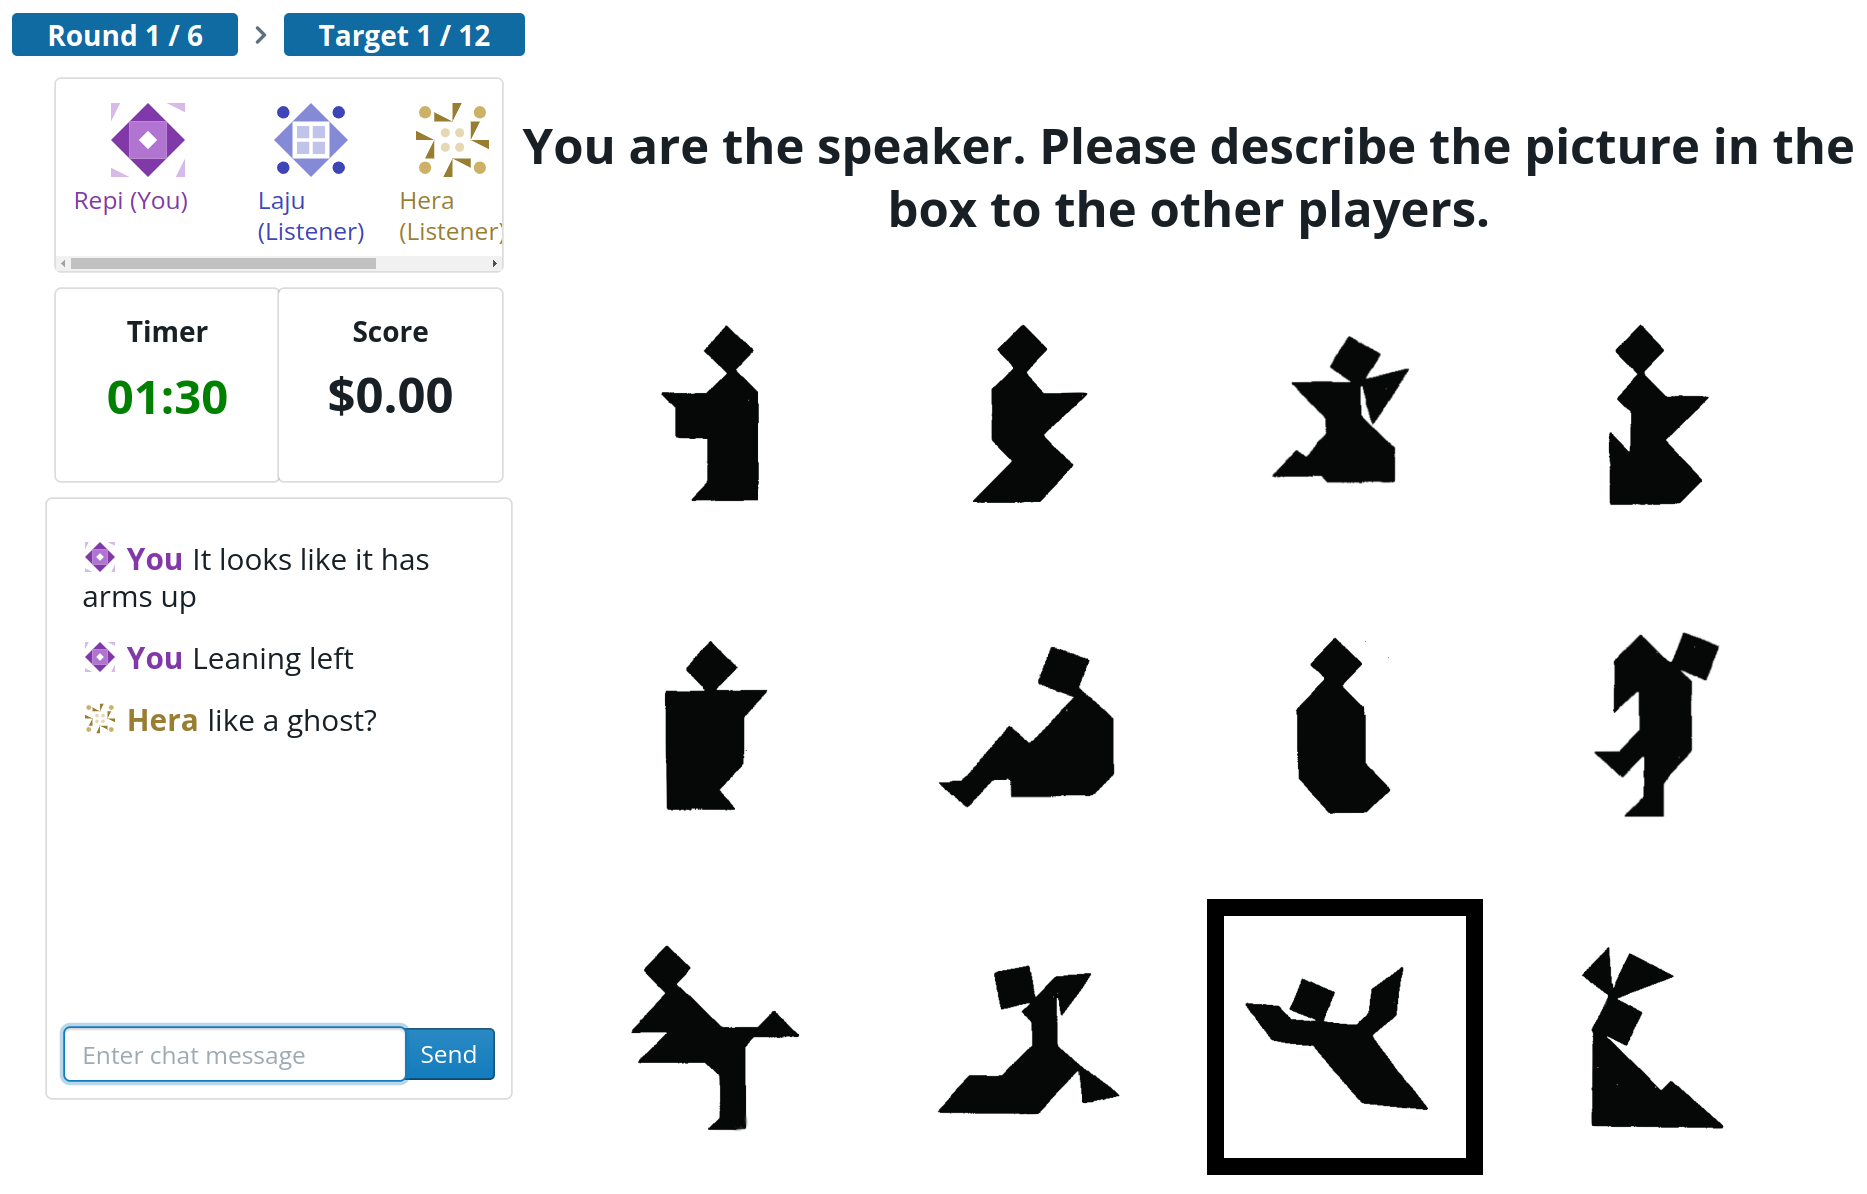
\includegraphics[width=20em]{images/diagram.png}};

		
		\node[illus, anchor=north west, minimum width=25em, minimum height=19em, ultra thick] (block) at (\ax+7.5, \ay+3) {};
		\node[illus, anchor=north west, minimum width=22em, minimum height=15em, ultra thick] (block) at (\ax+8, \ay+2.2) {};
		\node[anchor=north] () at (\ax+13, \ay+3.5) {Experiment (x 6 blocks)};
				\node[anchor=north] () at (\ax+13, \ay+2.8) {Block (x 12 trials)};
						\node[anchor=north] () at (\ax+13, \ay+1.8) {Trial};





%	\node[bound, ultra thick, anchor=north, minimum width=50em, minimum height=17em] (block) at (6.5, -5.5) {};
		
	\node[toplabel, align=center, anchor=north] at (\colb,\clabx) {Matcher Contributions};
	 \node[illus, anchor=north, minimum width=12em] () at (\colb,\claby) {Emoji \\ 
\includegraphics[height=3.5em]{images/nochat.png}};
	 \node[illus, anchor=north, minimum width=12em] () at (\colb,\clabz) {Chat \\ 
\includegraphics[height=3em]{images/chat.png}};
	 	
	 	
	 
	 
	\node[toplabel, align=center, anchor=north] at (\cola,\clabx) {Group  Size};
		\node[illus,anchor=north, minimum width=7em] () at (\cola,\claby) {Two person \\ 
\includegraphics[height=3em]{images/two.png}};
		\node[illus, anchor=north, minimum width=7em] () at (\cola, \clabz) {Six person \\ 
\includegraphics[height=3em]{images/six.png}};
		

 \node[toplabel, align=center, anchor=north] at (\colc/2+\cold/2,\clabx) {Group  coherence};		 

	
\node[align=center, anchor=north] at (\colc, \clabx-.9) {Describer rotation};

	\node[illus, anchor=north, minimum width=12em] () at (\colc,\claby) {Rotating describer\\ 
\includegraphics[height=4em]{images/rotate.png}};
	\node[illus, anchor=north, minimum width=12em] () at (\colc, \clabz) {Same describer\\ 
\includegraphics[height=4em]{images/norotate.png}};	

		 

	\node[align=center, anchor=north] at (\cold, \clabx-.9) {Task Feedback};
	
	\node[illus, anchor=north, minimum width=10em] () at (\cold,\claby) {Limited feedback\\ 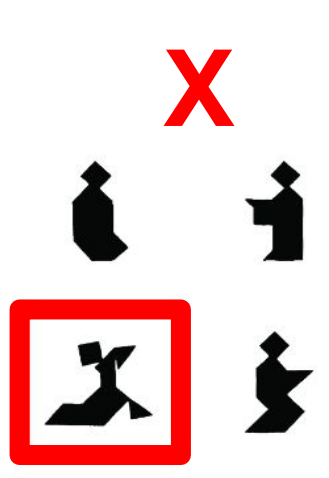
\includegraphics[height=5em]{images/limited-wrong.png} 
\phantom{m} 
\includegraphics[height=5em]{images/limited-correct.png}};



	\node[illus, anchor=north, minimum width=10em] () at (\cold, \clabz) {Full feedback \\  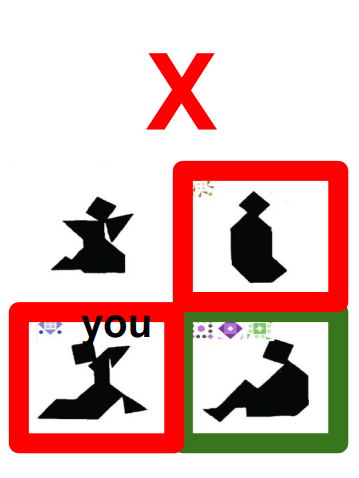
\includegraphics[height=5em]{images/full-wrong.png}  \phantom{m} 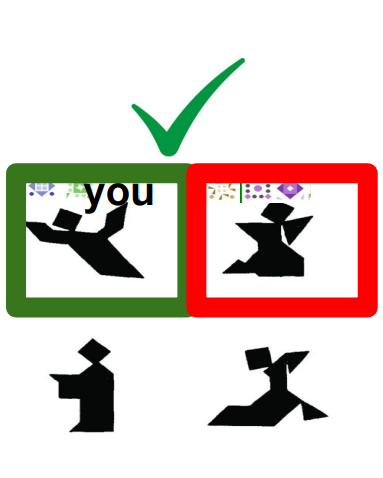
\includegraphics[height=5em]{images/full-correct.png}	};


		

		
		
		
	\end{tikzpicture}
	




	

\end{document}